\section{电磁波的辐射}
对应电动力学课本第五章,占分10分左右。

\begin{question}
    已知一电偶极辐射势为:$\mathbf{A}^{(0)}(\mathbf{R},t)=\frac{\mu_0}{4\pi}\frac{\dot{\mathbf{p}}\exp (ikR)}{R}$的电偶极子,
    $\dot{\mathbf{p}}=\frac{1}{2} I_0 l \textbf{\textit{e}}_z$,竖直放在距地面为h处,$h \ll \lambda$,
     可将地面看作理想导体,试求其辐射场和平均辐射能流。
\end{question}

\begin{question}
    两根完全相同的直天线,长度为$l\ll \lambda$,
    在天线中点外接交变电动势,天线上电流为: $I(z,t)=I_0[1-\frac{2}{l}\left| z \right|]\textit{e}^{-i\omega t}$,
    天线并行排列,如图所示,相距为$a\ll \lambda$,计算辐射场、辐射角分布和辐射功率。
    \begin{figure}[ht]
        \centering
        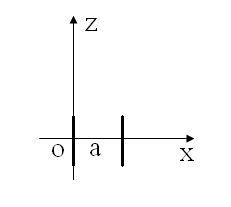
\includegraphics[height=3 cm]{images/q4_1.png}
        \caption{题\thequestion}
    \end{figure}
\end{question}

\begin{question}
    已知推迟势$\mathbf{A}(\mathbf{R},t)=\frac{\mu_0}{4\pi}\int \frac{\mathbf{J}(\mathbf{R}',t-r/c)}{r} \mathrm{d}V'$,
    假定周期变化的电流$\mathbf{J}(\mathbf{R}',t)=\mathbf{J}(\mathbf{R}')\textit{e}^{-i\omega t}$。当实际问题中的电流分布在一个小区域时,
    可用多极展开法来计算矢势。证明矢势展开的第一项与电偶极矩有关,
    即$\mathbf{A}^{(0)}(\mathbf{R},t)=\frac{\mu_0}{4\pi}\frac{\dot{\mathbf{p}}\exp (ikR)}{R}$,并给出矢势展开的第二项远远小于第一项的条件。
\end{question}

\begin{question}
    振荡的电偶极子的电磁场为:
    $$\mathbf{E}=\frac{\textit{e}^{ikR}}{4\pi\varepsilon_0 }\left \{ \frac{-k^2}{R}\mathbf{R}_0\times(\mathbf{R}_0\times \mathbf{p})+(\frac{ik}{R^2}-\frac{1}{R^3})(\mathbf{p}-3\mathbf{p}\cdot\mathbf{R}_0\mathbf{R}_0) \right \}$$
    $$\mathbf{B}=\frac{\mu_0 \omega }{4\pi c}(\frac{1}{R}-\frac{1}{ikR^2})\textit{e}^{ikR}\mathbf{R}_0\times \mathbf{p}$$
     其中$\mathbf{R_0}=\frac{\mathbf{R}}{R}$,$\mathbf{p}$为电偶极矩。
    
     \noindent (1)试写出场源近区和远区的解所满足的条件,分别推出近区和远区的电磁场。指出近区场和远区场的主要差别。
    
     \noindent (2)试推出远区的电磁场。将$\mathbf{p}$的位置选在坐标原点, 的方向选为z方向,写出$\mathbf{E}$和$\mathbf{B}$的具体形式。试求辐射场的平均能流(辐射角分布)以及辐射功率。
\end{question}

\begin{question}
    从麦克斯韦方程组出发引入变化电磁场的矢势$\mathbf{A}$和标势$\phi$,
    推出$\mathbf{A}$和$\mathbf{\phi}$满足的一般方程,并加入洛仑兹条件推出达朗伯方程。
\end{question}

\begin{question}
    由电偶极矩$\mathbf{p}$的定义及电荷连续性方程,
    证明:$$\frac{\mathrm{d} \mathbf{p}}{\mathrm{d} t}=\int_V \mathbf{J}\mathrm{d}V'$$    
\end{question}
